%!TEX root = ../main.tex

\chapter{Aufbau}
\label{ch:aufbau}

\section{Architektur}
\begin{figure}[ht]
    \centering
    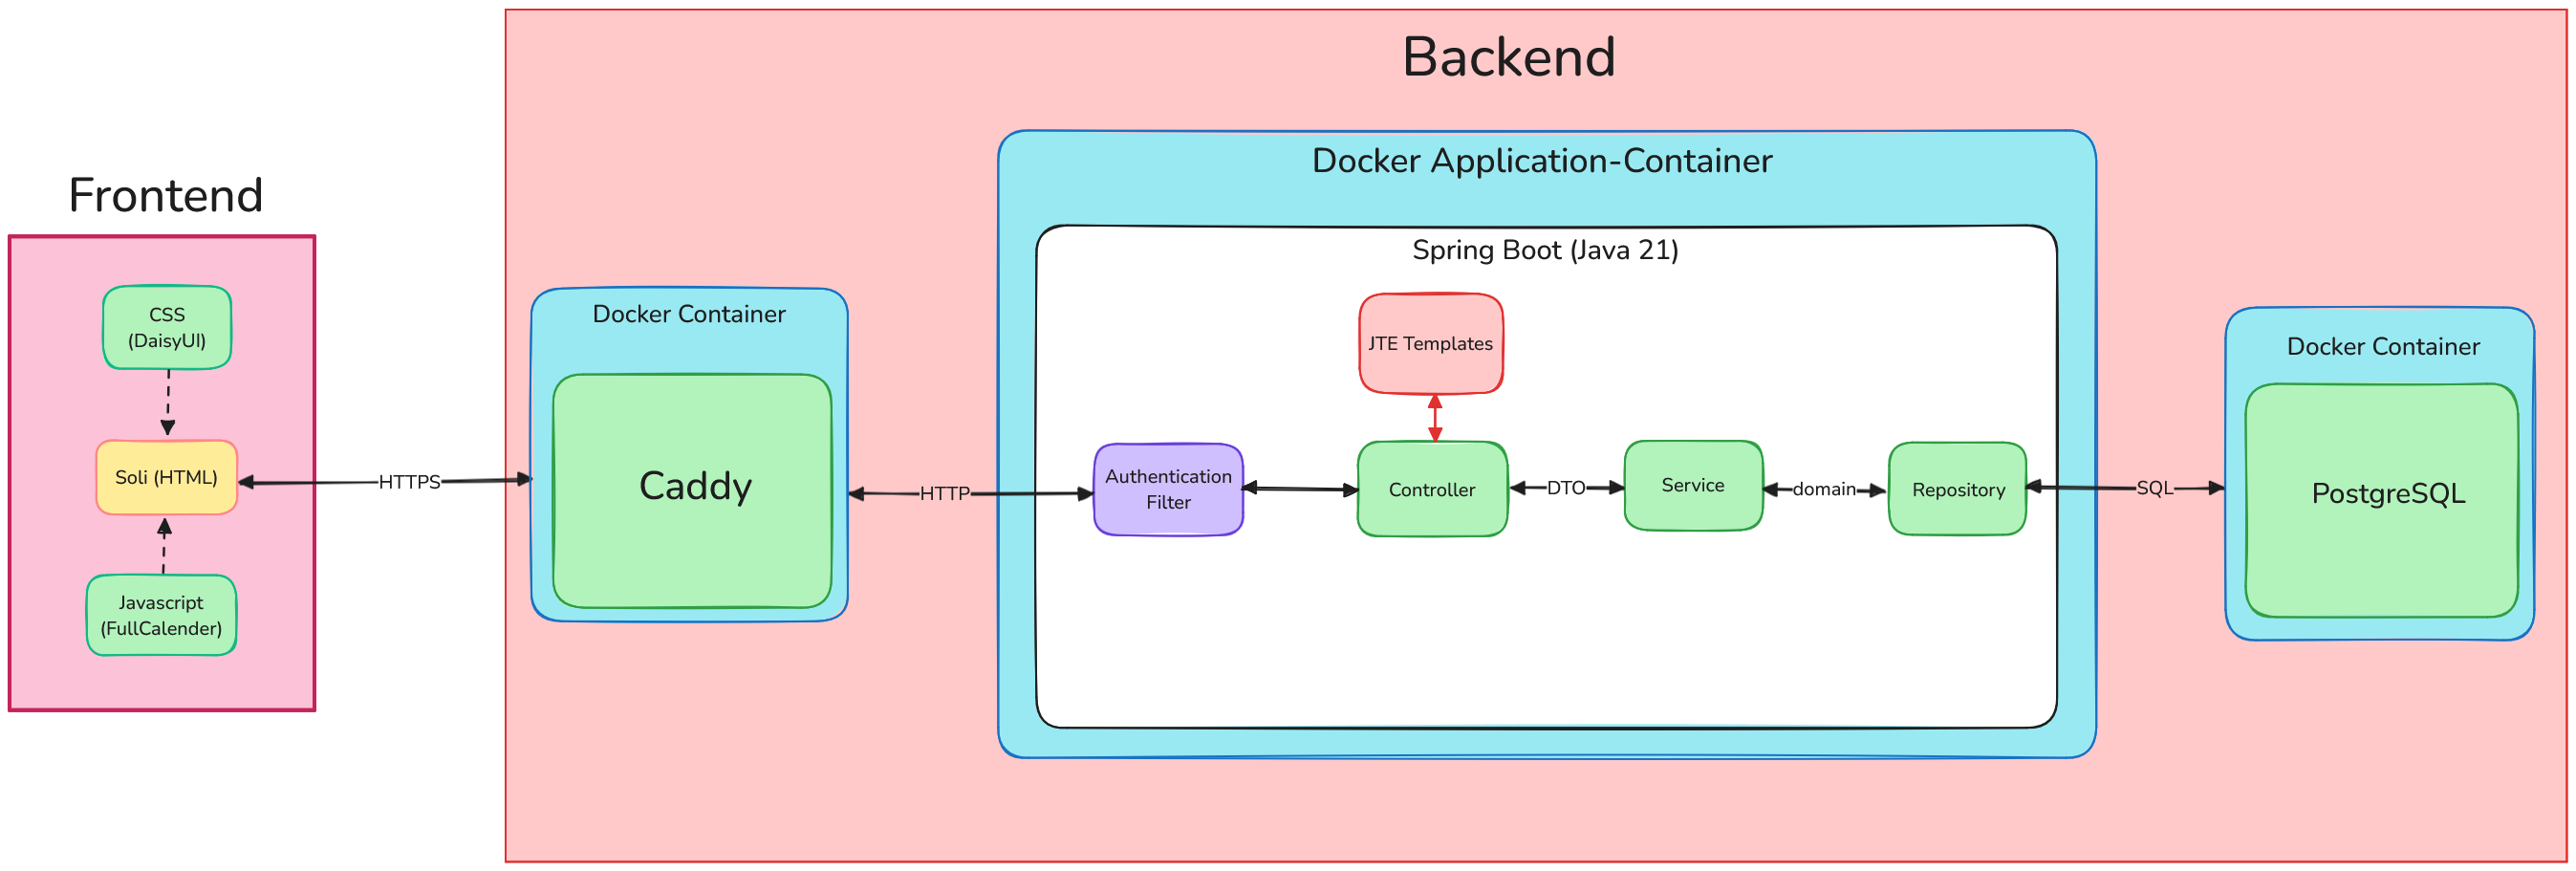
\includegraphics[width=\textwidth]{figures/architecture}
    \label{fig:architekturmodell}
\end{figure}
Die Architektur ist in \textit{Frontend} und \textit{Backend} unterteilt und folgt der \gls{MVC-Struktur} zur klaren Trennung der Verantwortlichkeitsbereiche.
Das \textit{Frontend} nutzt \gls{HTML}, \gls{DaisyUI} für das Design und \gls{FullCalendar} in \gls{JavaScript} für die Kalenderfunktionalität.
Die Kommunikation mit dem Backend erfolgt über \gls{HTTPS}.

Ein \gls{Caddy}-Server, welcher in einem eigenen \gls{Container} läuft, dient als \gls{HTTPS-Reverse-Proxy} und leitet Anfragen an das Backend weiter.
Das \textit{Backend} basiert auf \gls{Spring Boot} (Java 21) und läuft in einem weiteren \gls{Container}.
Dort prüft ein \textit{Authentication Filter} die Anfragen, die danach von einem \gls{Controller} verarbeitet werden.
Mithilfe von \gls{JTE}-Templates werden dynamische HTML-Antworten generiert.
Die \textit{Businesslogik} liegt in den \gls{Services}, die Anfragen koordinieren und weiterleiten.
Die \textit{Repositories} kapseln den SQL-Zugriff und ermöglichen eine saubere, abstrahierte Kommunikation
mit der \gls{PostgreSQL}-Datenbank in einem separaten \gls{Container}.

Der Einsatz von \gls{Docker} sorgt für eine einfache Bereitstellung und Wartbarkeit der Anwendung.
\clearpage

\section{Klassendiagramm}
\begin{figure}[ht]
    \centering
    \includegraphics[angle=90, height=1.1\textwidth]{figures/classes}
    \label{fig:klassendiagramm}
\end{figure}
\clearpage